
\nextchapter{Introduction to Analysis}
\begin{Definition}
\textbf{Norm} on LS $(V,F)$ is func $\fnorm{\cdot}{}:V\to\mathbb R_+\equiv\{x\in\mathbb R|x\ge 0\}$ s.t.
\begin{enumerate*}[label=\protect\circled{\arabic*}]
  \item[\circled{0}] Maps to $\mathbb R_+$ !!!
  \item $\forall v_1,v_2\in V,\fnorm{v_1+v_2}{}\le\fnorm{v_1}{}+\fnorm{v_2}{}$
  \item $\forall v\in V,\forall a\in F,\fnorm{av}{}=|a|\fnorm{v}{}$
  \item $\fnorm{v}{}=0\Leftrightarrow v=0$
\end{enumerate*}
\end{Definition}
\begin{Definition}
\textbf{Normed linear space} is $(V,F,\fnorm{\cdot}{})$.
\end{Definition}
\begin{center}
$\fnorm{x}{1}=\sum_i|x_i|\quad
\fnorm{x}{2}=\sqrt{\sum_i|x_i|^2}\quad
\fnorm{x}{\infty}=\max_i|x_i|$
\end{center}

\begin{Definition}
\textbf{\hl{(Open) ball}} in $(V,F,\fnorm{\cdot}{})$: $B(v,r)=\{v'\in V|\fnorm{v-v'}{}<r\}$. 
$B(0,1)$ \textbf{unit ball}.  $S\subseteq V$ \textbf{bounded} if $\exists r\in\mathbb R_+|S\subseteq B(0,r)$.

\textbf{Sequence} $\sequence{v}{i}{\infty}$ in $(V,F,\fnorm{\cdot}{})$ \textbf{converges} to $\bar v\in V\Leftrightarrow\forall\varepsilon>0\exists N\in\Naturals|\forall m\ge N,\fnorm{v_m-\bar v}{}<\varepsilon$.

Set $K\subseteq V$ \textbf{closed}$\Leftrightarrow$ contains all its limit points $\Leftrightarrow\forall\sequence{v}{i}{\infty}\subseteq K$, if $v_i\to v\in V$ then $v\in K$. $K$ is \textbf{open}$\Leftrightarrow$complement $V\setminus K$ closed. $K$ \textbf{compact} if both closed and bounded.

$f:U\to V$ \textbf{\hl{continuous at $u\in U$}} $\Leftrightarrow\forall\varepsilon>0\exists\delta>0\text{ s.t. }\fnorm{u-u'}{U}<\delta\Rightarrow\fnorm{f(u)-f(u')}{V}<\varepsilon$.
$f$ \textbf{cont on $U$}$\Leftrightarrow$cont $\forall u\in U$.
\end{Definition}
\begin{Theorem}
$\fnorm{\cdot}{a}$ \& $\fnorm{\cdot}{b}$ \textbf{equiv}$\Leftrightarrow\exists m_u\ge m_l> 0,m_l\fnorm{v}{a}\le\fnorm{v}{b}\le m_u\fnorm{v}{a}$
\end{Theorem}

\begin{Fact}
$x\in V$,$B_a(0,1)=\{\fnorm{x}{a}<1\}$, $B_b(0,1)=\{\fnorm{x}{b}<1\}$: $m_l\fnorm{x}{a}\le\fnorm{x}{b}\le m_u\fnorm{x}{a}\Rightarrow$\hl{$B_b(0,m_l)\subseteq B_a(0,1)\subseteq B_b(0,m_u)$}
\end{Fact}
\begin{Proof}
$x\in B_a(0,1)\Rightarrow\fnorm{x}{a}<1\Rightarrow\fnorm{x}{b}<m_u\Rightarrow x\in B_b(0,m_u)\Rightarrow B_a(0,1)\subseteq B_b(0,m_u)$.
$y\in B_b(0,m_l)\Rightarrow m_l\fnorm{x}{a}\le \fnorm{y}{b}<m_l\Rightarrow \fnorm{x}{a}<1\Rightarrow x\in B_a(0,1)\Rightarrow B_b(0,m_l)\subseteq B_a(0,1).$ \QED
\end{Proof}
\begin{minipage}{0.45\columnwidth}
$
\arraycolsep=1.4pt
\begin{array}{rcccl}
\fnorm{x}{2}&\le&\fnorm{x}{1}&\le&\sqrt{n}\fnorm{x}{2} \\
\textcolor{blue}{1}\cdot\textcolor{green}{\fnorm{x}{\infty}}&\le&\fnorm{x}{2}&\le&\textcolor{red}{\sqrt{n}}\textcolor{green}{\fnorm{x}{\infty}}\\
\fnorm{x}{\infty}&\le&\fnorm{x}{1}&\le& n\fnorm{x}{\infty}
\end{array}
$
\end{minipage}%
\begin{minipage}{0.07\columnwidth}
\begin{center}
\includegraphics[width=1\columnwidth]{figures/norm_bounded.pdf}
\end{center}
\end{minipage}%
\begin{minipage}{0.48\columnwidth}
\textbf{Schwarz's Inequality:}
\begin{center}
$\sum_{i=1}^n(|x_i|\cdot |y_i|)\le\fnorm{x}{2}\fnorm{y}{2}$
\end{center}
$\forall x,y\in F^n$.
\end{minipage}

\begin{Fact}
$\fnorm{\cdot}{a}$, $\fnorm{\cdot}{b}$ equiv. $\sequence{v}{i}{\infty}$ CV in $(V,F,\fnorm{\cdot}{a})\Leftrightarrow$CV in $(V,F,\fnorm{\cdot}{b})$.
\end{Fact}
\begin{Fact}
Open/closed sets remain open/closed $\forall$ equivalent norms.
\end{Fact}
\begin{Theorem}
\hl{Any 2 norms on a finite-dim space are equivalent!}
\end{Theorem}
\begin{Fact}
\textbf{Weierstrass} continuous $f:S\to\mathbb R$ defined on $S\subseteq\mathbb R^n$ that's compact in $(\mathbb R^n,\fnorm{\cdot}{2})$ attains a (non-($-\infty$)) \textbf{minimum} on $S$.
\end{Fact}
\nextsubchapter{Infinite-dim linear spaces}
\begin{center}
$
{
\fnorm{f}{1}\hspace{-1mm}=\hspace{-1mm}\int_{t_0}^{t_1}\fnorm{f(t)}{2}dt
,
\fnorm{f}{2}\hspace{-1mm}=\hspace{-1mm}\sqrt{\int_{t_0}^{t_1}\fnorm{f(t)}{2}^2dt}
,
\fnorm{f}{\infty}\hspace{-1mm}=\hspace{-1mm}\underset{[t_0,t_1]}{\max}\fnorm{f(t)}{2}
}
$
\end{center}
All $\fnorm{f}{i}$ not equiv. \hl{Proof: family} $f_n(t)=t^n\in C([0,1],\Reals)$, $n\in\Naturals$.

\begin{Definition}
\textbf{Cauchy seq} $\sequence{v}{i}{\infty}\Leftrightarrow\forall\varepsilon>0\exists N\in\Naturals,\forall m\ge N,\fnorm{v_m-v_N}{}<\varepsilon$
\end{Definition}
\begin{Fact}
Convergent sequence$\Rightarrow\nLeftarrow$Cauchy.
\end{Fact}
\begin{Definition}
$(V,F,\fnorm{\cdot}{})$ \textbf{complete} (\textbf{Banach})$\Leftrightarrow$all Cauchy seq's in it converge
\end{Definition}
\begin{Theorem}
Every finite-dimensional lin. space $(V,F)$ is Banach, for any $\fnorm{\cdot}{}$.
\end{Theorem}
$(\mathbb R,\mathbb R,\fnorm{\cdot}{})$ is Banach. $(C([t_0,t_1],\mathbb R^n),\mathbb R,\fnorm{\cdot}{\infty})$ is Banach.

\begin{Definition}
Let $f:(U,F,\fnorm{\cdot}{U})\to(V,F,\fnorm{\cdot}{V})$. \textbf{\hl{Induced norm}} of $f$:
\begin{equation*}
\fnorm{f}{}=\sup_{u\ne 0}\frac{\fnorm{f(u)}{V}}{\fnorm{u}{V}}
\end{equation*}
For lin maps $\linA:U\to V$, suffice: $\fnorm{\linA}{}=\sup_{\fnorm{u}{U}=1}\fnorm{\linA(u)}{V}$
\end{Definition}
$
\overset{\text{Induced norms of}}{\linA:F^n\to F^m}:\hspace{-1mm}
\begin{cases}
\fnorm{A}{1}=\max_{j=1,\ldots,n}\sum_{i=1}^m|a_{ij}| & \text{row sum} \\
\fnorm{A}{\infty}=\max_{i=1,\ldots,m}\sum_{j=1}^n|a_{ij}| & \text{col sum} \\
\fnorm{A}{2}=\max_{\lambda\in\Spec[A^TA]}\sqrt{\lambda} & \text{max eig.}
\end{cases}
$

\begin{Theorem}
Let \textit{linear} map $\linA:(U,F,\fnorm{\cdot}{U})\to(V,F,\fnorm{\cdot}{V})$. \textit{Equivalent}:
\begin{enumerate*}
  \item \hl{$\linA$ continuous}.
  \item $\linA$ continuous at 0.
  \item \hl{$\sup_{\fnorm{u}{U}=1}\fnorm{\linA(u)}{V}<\infty$} and induced norm $\fnorm{\linA}{}$ is well-defined.
\end{enumerate*}
\end{Theorem}
\begin{Corollary}
\hl{All lin. funcs. between \textbf{finite-dim.} spaces are continuous.}
\end{Corollary}
\begin{Theorem}
Let $\linA,\tilde\linA:(V,F,\fnorm{\cdot}{V})\to(W,F,\fnorm{\cdot}{W})$ and $\linB:(U,F,\fnorm{\cdot}{U})\to(V,F,\fnorm{\cdot}{V})$. Let $\fnorm{\cdot}{}$ be the induced norms.
\begin{enumerate*}[label=\protect\circled{\arabic*}]
  \item $\forall v\in V,\fnorm{\linA(v)}{W}\le\fnorm{\linA}{}\cdot\fnorm{v}{V}$
  \item $\forall a\in F,\fnorm{a\linA}{}=|a|\fnorm{A}{}$
  \item $\fnorm{\linA+\tilde\linA}{}\le\fnorm{\linA}{}+\fnorm{\tilde\linA}{}$
  \item $\fnorm{\linA}{}=0\Leftrightarrow\linA(v)=0\forall v\in V$ (zero map)
  \item $\fnorm{\linA\circ\linB}{}\le\fnorm{\linA}{}\fnorm{\linB}{}$
\end{enumerate*}
\end{Theorem}
\begin{Proof}
$\fnorm{\linA\circ\linB}{}=\sup\fnorm{(\linA\circ\linB)(u)}{W}\le\fnorm{\linA}{}\sup\fnorm{\linB(u)}{V}=\fnorm{\linA}{}\fnorm{\linB}{}$ \QED
\end{Proof}
\nextsubchapter{Ordinary Differential Equations}
\begin{Definition}
$u\in PC([t_0,t_1],\mathbb R^m)$ is \textbf{piecewise continuous (pwc)}$\Leftrightarrow$cont at all $t\in\mathbb R$ except finite set of \textbf{discontinuity points} $D\subseteq\mathbb R$.
\end{Definition}
\begin{Theorem}
Consider \hl{ODE}: $\dot x(t)=p(x(t),t)\in PC([t_0,t_1],\mathbb R^n)$ (i.e. pwc in $t$). $\phi:\Reals\to\Reals^n$ passing through $(t_0,x_0)\in\Reals\times\Reals^n$ \textbf{solution}$\Leftrightarrow$
\begin{itemize*}
  \item $\phi(t_0)=x_0$
  \item $\forall t\in\Reals\setminus D,\phi$ differentiable at $t$ \& $\dot\phi(t)=p(\phi(t),t)$
\end{itemize*}
\end{Theorem}
\begin{Definition}
$p:\Reals^n\times\Reals\to\Reals^n$ is \textbf{\hl{globally Lipschitz in $x$}} (simply: ``\textbf{\hl{Lipschitz}}'') $\Leftrightarrow\exists$ $k:\Reals\to\Reals_+$ pwc s.t. $\forall x,x'\in\Reals^n,\forall t\in\Reals,\fnorm{p(x,t)-p(x',t)}{}\le k(t)\fnorm{x-x'}{}$. $k(t)$ called \textbf{Lipschitz constant} of $p$ at $t\in\Reals$.
\end{Definition}
\begin{Fact}
Are globally Lipschitz:
\begin{enumerate*}
  \item All linear functions
  \item All \textbf{differentiable} functions with \textbf{bounded derivatives}
\end{enumerate*}
\end{Fact}
Lipschitz $\Rightarrow\nLeftarrow$ continuous. Lipschitz $\nRightarrow$ differentiable.

\begin{Definition}
\textbf{Differentiable} func $f(x)$ is s.t. $df/dx$ exists/is well-defined $\forall x$.

Diffbl $\Rightarrow\nLeftarrow$ cont $\forall x\in D$. Reason: \begin{tikzpicture}
\draw (0,0) arc (-90:0:1mm);
\draw (1mm,1mm) arc (-180:-90:1mm);
\end{tikzpicture}, \begin{tikzpicture}
\draw (0,0) arc (-90:0:0.7mm);
\draw (0.7mm,0.7mm) arc (180:90:0.7mm);
\end{tikzpicture}, cont but not diffbl.

Multivar func diffbl $\Leftrightarrow$ Jacobian well-defined $\forall x\in D$.
\end{Definition}
\begin{Proof}
Methods to prove Lipschitzianity:
\begin{enumerate*}
  \item[\squaredcolornobord{M1}{yellow}] Show that derivative/Jac. bounded.
  \item[\squaredcolornobord{M2}{yellow}] Show that function linear.
  \item[\squaredcolornobord{M3}{yellow}] FTSOC, suppose $\exists k$ s.t. $|\sqrt x-\sqrt y|\le k|x-y|$. Take $x=1/n,y=0\Rightarrow(\sqrt{1/n}-\sqrt 0)/(1/n-0)=\sqrt n\Rightarrow\sqrt n\le k$. $k$ const in $n$, letting $n\to\infty$ contradic.! $\sqrt{x}$ not Lipschitz. \QED
\end{enumerate*}
\end{Proof}
\begin{Theorem}
Solution $\phi(t)$ to ODE $\dot x(t)=p(x(t),t)$ \hl{\textbf{exists} \& is \textbf{unique}} if $p$ pwc wrt $t$ and globally Lipschitz wrt $x$ (\textit{sufficient but not necessary!}). $\phi(t)$ is \textbf{pwc} e.g. \includegraphics[height=2ex]{figures/pwc.pdf}.
\end{Theorem}
\begin{Fact}
$\forall\fnorm{\cdot}{}$ on $\Reals^n$, $\forall t_0,t_1\in\Reals$: $\fnorm{\int_{t_0}^{t_1}f(t)dt}{}\le\left| \int_{t_0}^{t_1}\fnorm{f(t)}{}dt \right|$
\end{Fact}
\begin{itemize*}
  \item $\forall m,k\in\Naturals,(m+k)!\ge m!\cdot k!$
  \item $\forall c\in\Reals,\lim_{m\to\infty}[c^m/m!]=0$
\end{itemize*}

\begin{Theorem}
\textbf{Fund thrm calculus}. Let $g:\Reals\to\Reals$ pwc w/ disc set $D\subseteq\Reals\Rightarrow\forall t_0\in\Reals,f(t)=\int_{t_0}^t g(\tau)d\tau$ cont and $\forall t\in\Reals\setminus D,\frac{d}{dt}f(t)=g(t)$.
\end{Theorem}
\begin{Theorem}
\textbf{Leibniz}:
$
\frac{d}{dt}\left[\int_{a(t)}^{b(t)}f(t,\tau)d\tau\right]=
\int_{a}^{b}\frac{\partial f(t,\tau)}{\partial t}d\tau+f(t,b)\dot b-
f(t,a)\dot a
$
\end{Theorem}
\begin{Theorem}
\textbf{Gronwall Lemma}. Let $u(\cdot),k(\cdot):\Reals\to\Reals_+$ pwc, $c_1\ge 0,t_0\in\Reals$. $\forall t,u(t)\le c_1+\left| \int_{t_0}^{t}k(\tau)u(\tau)d\tau \right|\Rightarrow \forall t, u(t)\le c_1\exp\left| \int_{t_0}^t k(\tau)d\tau \right|$

\begin{Example}
$-k\fnorm{s(t,t_0,x_0)-\hat x}{}\le \frac{d}{dt}\fnorm{x(t,t_0,x_0)-\hat x}{}\le k\fnorm{s(t,t_0,x_0)-\hat x}{}$

$\Rightarrow \fnorm{x_0-\hat x}{}e^{-k(t-t_0)}\le \fnorm{s(t,t_0,x_0)-\hat x}{}\le \fnorm{x_0-\hat x}{} e^{k(t-t_0)}$
\end{Example}
\end{Theorem}
